\chapter{Approach}
\index{Approach%
@\emph{Approach}}%

This chapter discusses the architectural approach taken to implement Speakur\index{Speakur}, 
a social discussion plugin for the desktop and mobile web based on Web Components\index{Web Components} and the Polymer\index{Polymer} framework.

\section{Functionality}
Speakur\index{Speakur} 
is a Custom Element\index{Custom Elements} 
(\tcode{<speakur-discussion>}\index{<speakur-discussion>}) 
that provides a drop-in discussion forum or comment hosting service for a blog, web page or other web application.
An example of the user interface\index{user interface} can be found in Figure~\ref{f:demo1}.
Placing Speakur inside a web resource is very straightforward.
As shown in Listing~\ref{l:example1},
and in section \ref{publishing} below,
you simply place the \tcode{<speakur-discussion>}\index{<speakur-discussion>}
 element in your page's HTML at the desired spot.
This requires two supporting steps described in detail in section \ref{publishing}:
\begin{itemize}
\item loading the Web Components polyfill\index{polyfill} library script
\item importing the \tcode{<speakur-discussion>}\index{<speakur-discussion>} element.
\end{itemize}

Having done that, your web page now has an integrated discussion forum that works equally well for desktop and mobile users. 
All forum data including user profiles and comment text is stored in an online cloud database called Firebase~\cite{firebasecontributors2015}\index{Firebase}.
The encapsulated\index{encapsulation} nature of Speakur means that the messy details of structuring a discussion forum are hidden from its users.

\tcode{<speakur-discussion>}\index{<speakur-discussion>} presents a simplified interface (API)\index{API} to users.
There are only a few options to set including the URL of the Firebase instance and the thread target URL or \tcode{href}\index{href}.
If you do not provide your own a Firebase\index{Firebase} URL, by default, my own resource-limited database is used instead.
Therefore serious users will wish to use their own Firebase account and instance.

In addition to basic commenting features, Speakur offers the ability to vote comments up or down, custom profiles, 
the ability to leave comments in Markdown\index{Markdown} syntax~\cite{githubcontributors2015} with syntax highlighting\index{syntax highlighting} for common programming languages, 
and (rough) user interface translations 
(localizations\index{localization}\index{internationalization}) 
in 15 languages as shown in Figure~\ref{f:lang}.

\begin{figure}[htb]
\centering
 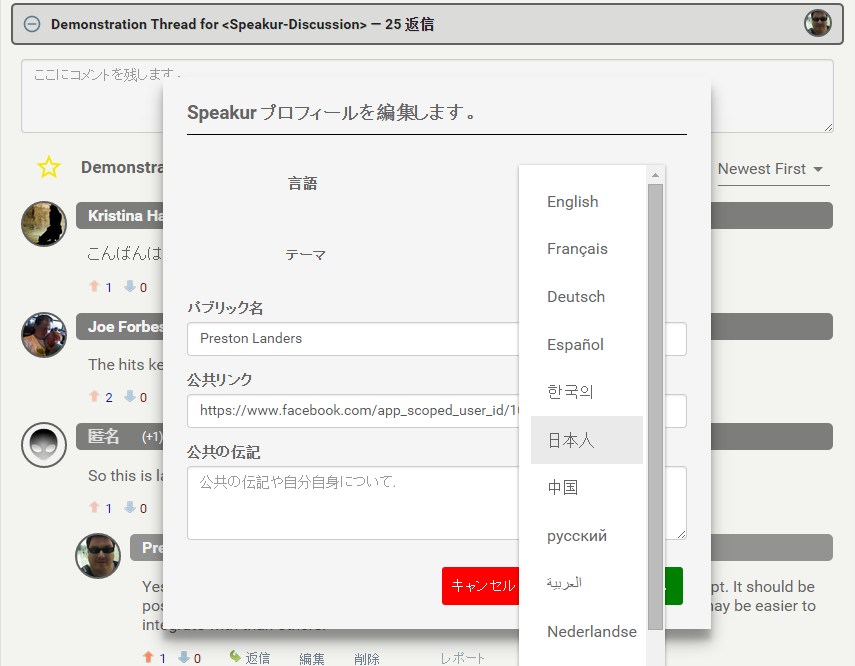
\includegraphics[width=5.5in]{images/screenshot_20150320_1923_lang.png}
\caption{Speakur's interface language\index{internationalization} updates instantly upon selection.}
\label{f:lang}
\end{figure}


From a technical perspective, one of Speaker's more interesting features is the use of Polymer's data-bound templates\index{data-bound template}, also known as Model-Driven Views\index{Model-Driven View}, 
to allow components to automatically reflect changes in far-flung areas of the application.
Also, Firebase's\index{Firebase} event notification\index{event notification} architecture allows all web clients to instantly and transparently reflect any changes in another remote client.
Another example of the power of data-bound templates is that all of the user-visible text in the application updates immediately as soon as the user changes his or her locale preference in the dialog in Figure~\ref{f:lang}.

\section{Architecture Overview}
It has been said that ``any problem in computer science can be solved with another layer of indirection\index{indirection}'' (usually attributed to Wheeler).
The key to understanding a software package is learning its architecture\index{architecture},
which is really a map of these layers of indirection\index{indirection} and abstraction\index{abstraction}.
Roy Fielding, the author of the influential REST web architecture, described a software architecture as:

\begin{quote}
\dots an abstraction of the run-time elements of a software system during some phase of its operation. A system may be composed of many levels of abstraction and many phases of operation, each with its own software architecture.

At the heart of software architecture is the principle of abstraction: hiding some of the details of a system through encapsulation\index{encapsulation} in order to better identify and sustain its properties. A complex system will contain many levels of abstraction, each with its own architecture~\cite{fielding2000}.
\end{quote}

The architecture for Speakur is based on client-side (browser) Javascript code and HTML layout following Web Components design principles. 
There is no server component at all except for the Firebase.com service~\cite{firebasecontributors2015}\index{Firebase}.
The software is built entirely out of plain HTML, JS and CSS\index{CSS} files that can be served from a static web host such as \tcode{github.io}~\cite{landers2015-d}.

Most of the main user interface elements in Speakur\index{Speakur} --- things like dropdown menus and dialogs as well as invisible functional components like expand/collapse elements  --- are provided by Polymer's\index{Polymer} Core\index{Core Elements} and Paper\index{Paper Elements} custom element libraries.
Speakur presents a simple external API around \tcode{<speakur-discussion>}\index{<speakur-discussion>},
but internally it consists of a number of internal abstraction layers or custom elements.
In turn, these internal layers consist of still more focused layers, other Polymer components, simple HTML templates, and wrappers around external Javascript libraries like  \tcode{moment.js}\index{moment.js library}.

This low-overhead design allows Speakur\index{Speakur} to be used on your own website without actually `installing' any software;
just load Speakur directly from \tcode{github.io} with an \textit{import}~\cite{landers2015-d}
and then insert a tiny bit of HTML into your document.
As previously mentioned, in order to make the 
\tcode{<speakur-discussion>}\index{<speakur-discussion>} element available for use, you must first load the Web Components polyfill\index{polyfill} and then \textit{import} the Speakur element, either from \tcode{github.io} or your own server.
It is recommended to create your own Firebase\index{Firebase} instance for data security and resource limitation reasons, but even this is not required. 
The author's demonstration database will be used by default.


Security\index{security} for web clients engaging in data manipulation (i.e, posting, editing or deleting comments) is handled entirely through Firebase\index{Firebase} authentication\index{authentication} and data security\index{security} rules described below.
The simplicity of this arrangement means that it is extremely easy to fit Speakur into almost any web application architecture.

\section{Responsive Design}
Because Speakur\index{Speakur} is not a standalone application but rather a plug-in designed to be embedded into other web pages or apps, 
the full document is not under its control.
This can affect the mobile\index{mobile} user experience\index{user experience (UX)},
but within these limits, Speakur strives to present a responsive\index{responsive} interface to different screen sizes.

The primary way it does this is...

\section{Polymer and Web Components}
As described in the Background chapter, Web Components\index{Web Components} are a W3C\index{W3C} initiative to expose certain native browser features in a public, standardized way. 
Polymer\index{Polymer} is a Google\index{Google} web framework built from the ground up around Web Components.

In general, Speakur tries to adhere to the core principles laid out by the 
Web Components\index{Web Components} developers 
for general purpose components~\cite{webcomponentscontributors2014}. 
It's worth reproducing those here in full:
\begin{quote}
\begin{itemize}
\item Address a common need.
\item Do one job really well.
\item Work predictably in a wide variety of circumstances.
\item Be useful right out of the box.
\item Be composable.
\item Be styleable.
\item Be extensible.
\item Think small.
\item Adapt to the user and device.
\item Deliver the key benefit to HTML authors, not just coders.
\end{itemize}
\end{quote}

Explain how I follow those guidelines... [TODO]

\section{Data store and synchronization}
As mentioned, all persistent data is stored in a cloud database called Firebase~\cite{firebasecontributors2015}\index{Firebase}.
Anyone who wants to use Speakur\index{Speakur} can register for a free account on \tcode{firebase.com} and create a database instance to hold Speakur data.
No other server component is required.
Firebase is a NoSQL\index{NoSQL}-style key-value data store of the kind that has been popularized
with the growth of 
Node.js\index{Node.js}, a server-side Javascript\index{Javascript} environment,
and the MongoDB\index{MongoDB} NoSQL database~\cite{dickey2014}.

Firebase\index{Firebase} provides Web~Socket\index{Web Socket}-based event notification and synchronization 
as well as a JSON-based\index{JSON} security rule description format for securing\index{security} and validating user actions.

\subsection{NoSQL and Firebase}
Firebase\index{Firebase} can be used `standalone' as the sole provider of data services to an application, as Speakur does, or else it can be used as an auxiliary to other services or REST\index{REST} APIs\index{API}.

Firebase itself provides a REST API for data access.
The term REST or RESTful is abused quite a bit in the industry [CITE]
but in Roy Fielding's original 2000 Ph.D. thesis, 
REST refers primarily to transferring \textit{representations} of application state.
Specifically...

More about FB...


\subsection{Web Sockets}
Web Socket\index{Web Sockets} are a TCP/IP protocol that can be used alongside HTTP for persistent data connections between web clients and servers.
The primary purpose is to avoid the overhead of initiating a new HTTP connection to check on the status of something on the server, also known as polling\index{polling}.
Firebase\index{Firebase} uses Web Sockets rather than traditional high-overhead HTTP requests to move data back and forth to the client.
This always-on connection allows for sending nearly instant event notifications to all currently active clients with minimal overhead.
In practice, this allows the application to update its distributed state in real-time.

[CITE] for websockets?

\subsection{Security}
Firebase implements the two major categories of user access control: authentication and 
authorization~\footnote{
Authentication (sometimes abbreviated \textit{authn}) answers the question ``are you who you say you are?'' 
while authorization (\textit{authz}) asks ``what are you allowed to see and do?''}.

[CITE: Stallings]

\subsubsection{Authentication}

\subsubsection{Authorization}


\section{Data Flow and Event Handling}

\subsection{Mutation Observers}

\section{Dependencies and Deployment}

Bower\index{Bower}

Vulcanize\index{Vulcanize}

CORS\index{Cross-origin resource sharing (CORS)}

